Dans cette section nous appliquons le modèle de transport et
dissolution d'alumine en fonction de la température proposé dans la
section \ref{sec:populations-model} dans le cadre d'une cuve
d'électrolyse industrielle. Nous utiliserons la cuve AP32, qui
exploite la technologie de cuve d'électrolyse AP
Technology\texttrademark\ développée par RioTinto. Les premières cuves
basées sur la technologie AP ont été mises en production au début des
années 1990, et plus de \num{4000} d'entre elles fonctionnent encore
actuellement en production \cite{RiotintoAP30}. Nous commençons par
présenter le design et le mode d'opération de la cuve AP32. Nous
détaillerons ensuite le choix des différentes données qui
interviennent dans modèle numérique proposé dans la section
\ref{sec:populations-discretisation} et dans le cadre de la cuve
AP32. Finalement, nous présenterons une sélection de résultats
numériques obtenus.


% detail des aspects importants de l'operation d'une cuve
% d'electrolyse:
%  - geometrie de la cuve (taille, nombre d'anodes, epaisseur de bain
%    et de metal,
%  - alimentation electrique
%  - etat stationnaire de l'ecoulement, interface. remarque sur les
%    talus.
%  - control de la concentration d'alumine
%  - schema d'injection periodique, position des injecteurs
%  - calcul de la conductivite sigma du bain
%  - conditions initiales
%  - informations sur le post-processing et la visualisation.

\paragraph{Géométrie de la cuve AP32} La structure de la cuve AP32
occupe au sol une longueur d'environ \num{17} \si{\meter} et une
largeur d'environ \num{7} \si{\meter}. L'ensemble de la structure
s'élève sur environ \num{5} \si{\meter}. A l'intérieur de la cuve, les
fluides s'étendent sur environ
\num{14} \si{\meter}$\times$\num{3.5} \si{\meter}. L'épaisseur de la
couche d'aluminimum liquide en contact avec la cathode est d'environ
\num{17} \si{\centi\meter}, tandis que l'épaisseur maximale du bain
électrolytique, au niveau des canaux entre les blocs anodiques, est
d'environ \num{20} \si{\centi\meter}. L'ACD est typiquement de l'ordre
de \num{3} \si{\centi\meter}. Ces différentes épaisseurs varient d'un
point à l'autre de la cuve à cause des écoulements dans les fluides,
de la déformation de l'interface bain-métal et des irrégularités à la
surface des anodes. De plus, le volume de métal liquide varie
constamment, d'une part à cause du produit de la réaction
d'électrolyse, et d'autre part à cause des opérations de siphonnage du
métal, qui interviennent environ une fois par jour.

\begin{figure}[t]
  \begin{center}
    \begin{subfigure}[b]{0.49\textwidth}
      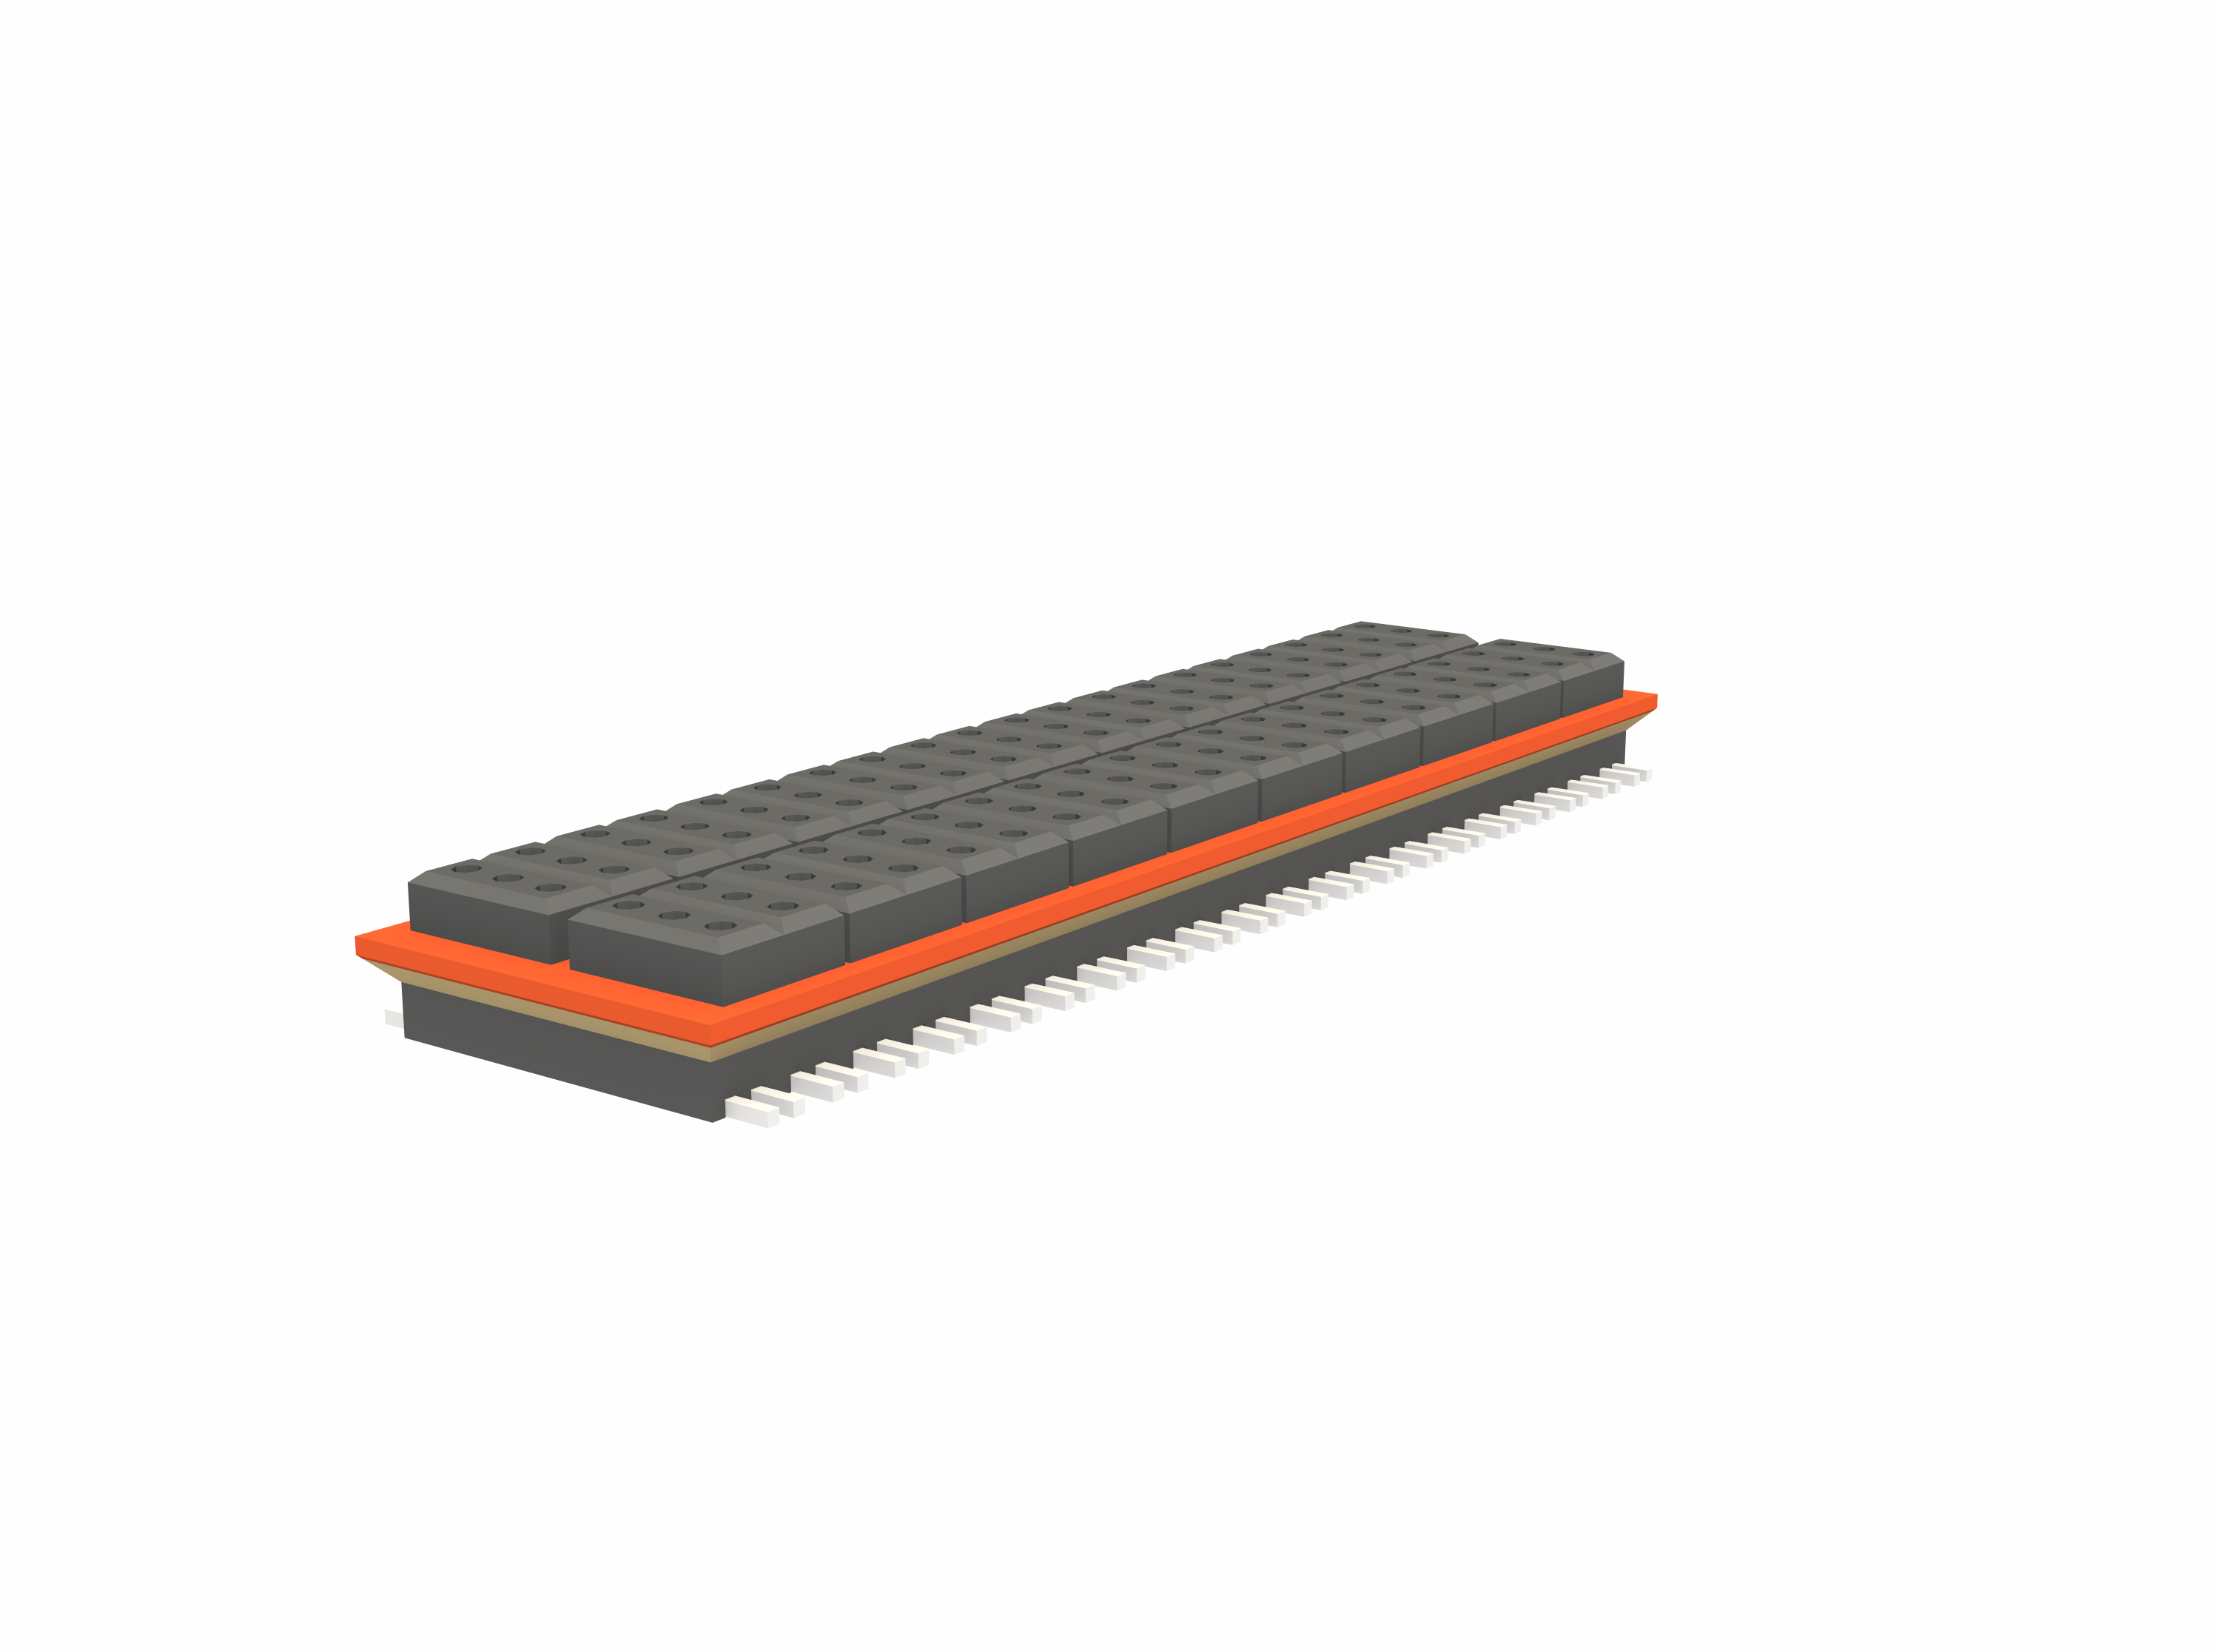
\includegraphics[width=\textwidth]{../media/populations/ap32-mesh-components/print/metal-bath-anodes-cathode-bus-bars.png}
      \caption{Éléments à proximité des fluides}

      \label{fig:ap32-geometry-bath}
    \end{subfigure}
    \begin{subfigure}[b]{0.49\textwidth}
      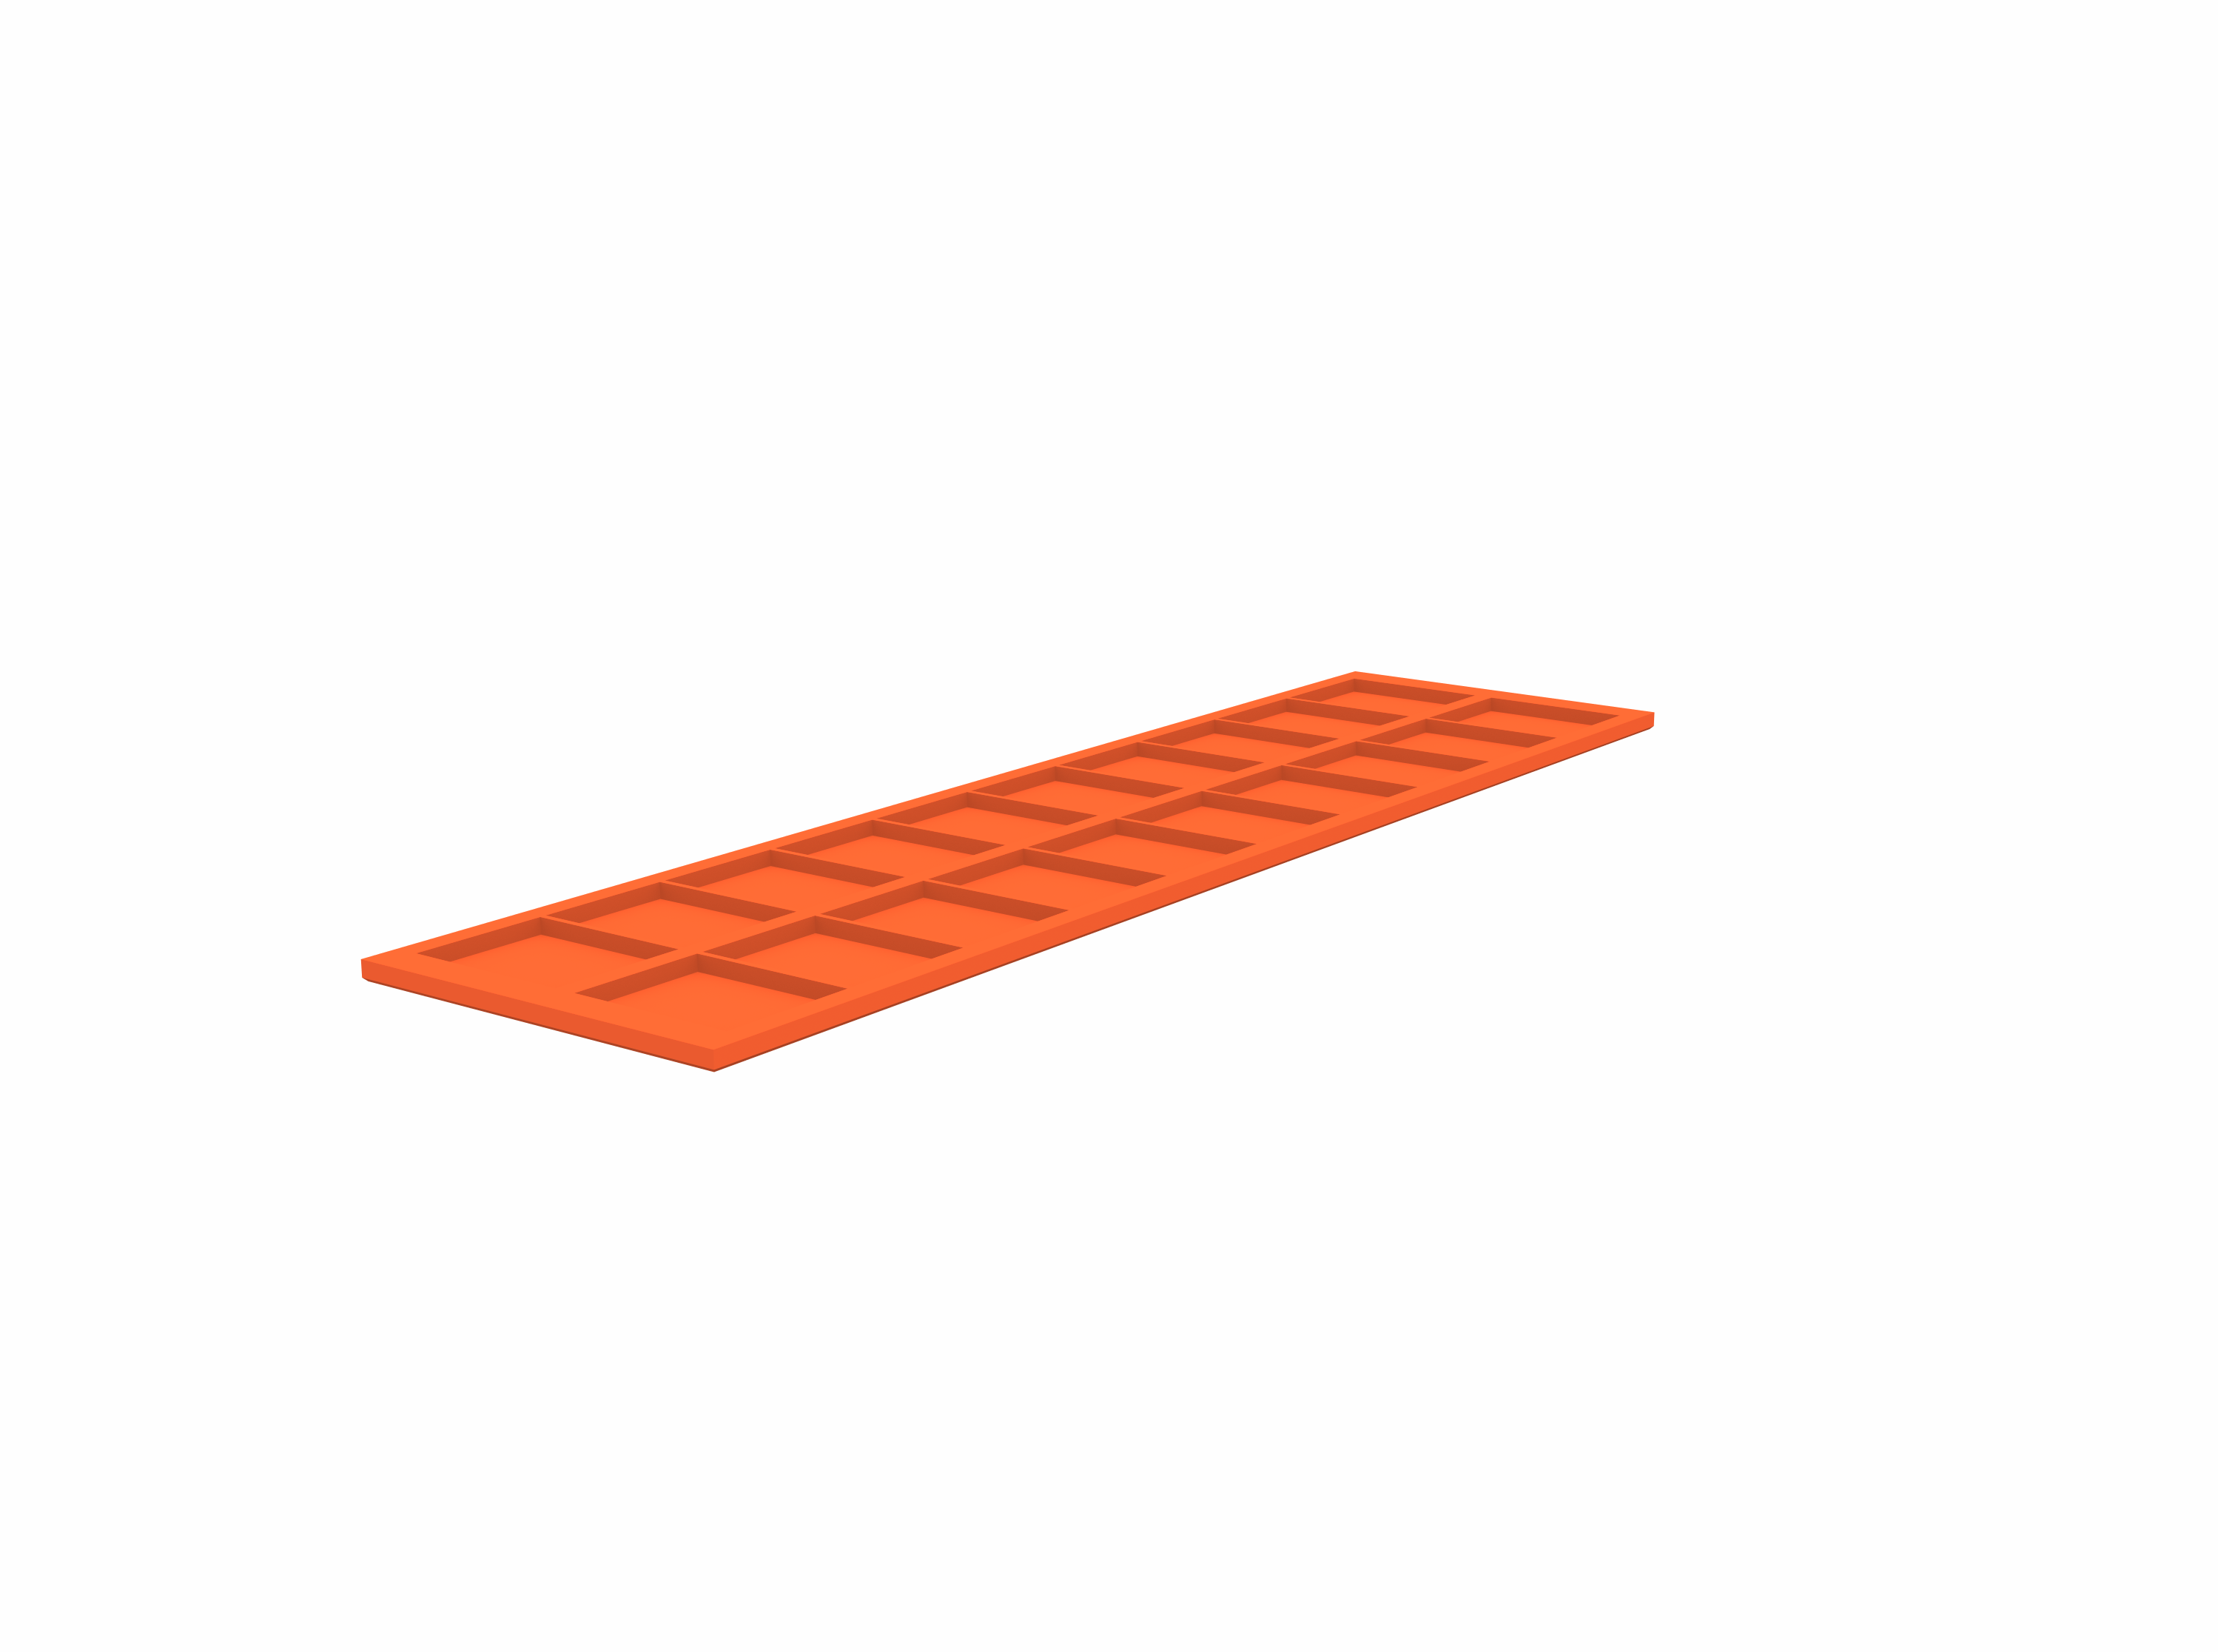
\includegraphics[width=\textwidth]{../media/populations/ap32-mesh-components/print/bath.png}
      \caption{Bain électrolytique}
      \label{fig:ap32-geometry-electrolyte}
    \end{subfigure}
    \caption{Géométrie des éléments importants à proximité
      du bain électrolytique dans une cuve AP32
      (fig. \ref{fig:ap32-geometry-bath}), et detail du volume
      occupé par le bain électrolytique dans cette même cuve
      (fig. \ref{fig:ap32-geometry-electrolyte}). On distingue les
      différentes partie suivantes: les anodes en haut et la cathode
      en bas (\textbf{noir}), le bain électrolytique
      (\textbf{orange}), le métal liquide (\textbf{orange}) et les
      bus bar (\textbf{gris clair}).  Les indentation rectangulaire
      á la surface du bain visibles dans la figure
      \ref{fig:ap32-geometry-bath} correspondent aux anodes
      partiellement immérgées dans celui-ci.}
    \label{fig:ap32-geometry}
  \end{center}
\end{figure}

Le plan anodique est composée de deux rangées de 10 anodes chacune.
